\section{The Lambert threshold, and why it is auxiliary}
\label{sec:lambert}

This section reports a negative result about our own starting point.

The Lambert $W$ function motivated the original formulation of this work, and it
is mathematically correct everywhere we use it. But the balance that justifies
$W$ turns out not to be the balance governing the system we actually integrate.
We could have quietly kept the boundary and let it look like a property of the
dynamics. We would rather set the whole thing out, because noticing this kind of
gap is exactly what separates a model you can use from mathematics you can
admire.

\subsection{When $W$ is actually required}

The Lambert $W$ function is defined implicitly by $W(y)e^{W(y)} = y$, and you
need it precisely when an unknown shows up both inside and outside an
exponential \citep{corless1996}. A relation
\begin{equation}
  x e^{x} = y \quad\Longrightarrow\quad x = W(y)
\end{equation}
genuinely requires it. A relation $e^{x} = y$ does not; that is a logarithm. Any
appearance of $W$ that does not rest on the first structure is decoration.

\subsection{The natural balance does not need $W$}

Take the Lambert recursion kernel $F(\Icap) = \Icap e^{\Icap}$ from
Table~\ref{tab:registry}. Equation~\eqref{eq:dI} becomes
\begin{equation}
  \dd{\Icap}{\tau} = a A \Icap + b \Arec \Icap e^{\Icap} - c \Reg \Icap - s_I \Icap^{2}.
\end{equation}
Set recursive amplification against regulatory damping, drop ordinary growth and
saturation for the moment, and you get
\begin{equation}
  b \Arec \Icap e^{\Icap} \;=\; c \Reg \Icap .
\end{equation}
Now look at what happens. For $\Icap > 0$ the factor $\Icap$ \emph{cancels on
both sides}, and we are left with
\begin{equation}
  b \Arec e^{\Icap} = c \Reg
  \qquad\Longrightarrow\qquad
  \Icap_{\mathrm{thr}} = \ln\!\left(\frac{c \Reg}{b \Arec}\right),
  \label{eq:logthreshold}
\end{equation}
a \emph{logarithmic} threshold. The Lambert structure is destroyed by the very
cancellation that the $\Icap e^{\Icap}$ kernel appeared to guarantee. The
damping term carries a factor of $\Icap$ too, and the two factors annihilate.
This is the central observation of the section, and it is remarkably easy to
miss --- we missed it for a while.

\subsection{Recovering Lambert structure requires a different balance}

Lambert structure survives only if $\Icap e^{\Icap}$ is set against a regulatory
capacity that is \emph{not} itself proportional to $\Icap$. Introduce such a
capacity,
\begin{equation}
  C_R \;=\; c\,\Reg^{\eta}\,\ln(1 + \Aref)\,\mathcal{E},
  \label{eq:CR}
\end{equation}
with $\eta$ a regulation exponent and $\mathcal{E}$ an alignment factor, impose
$b \Arec \Icap e^{\Icap} = C_R$, and now nothing cancels:
\begin{equation}
  \Icap e^{\Icap} = \frac{C_R}{b \Arec}
  \qquad\Longrightarrow\qquad
  \boxed{\;\Icrit \;=\; W\!\left(\frac{c\,\Reg^{\eta}\,\ln(1+\Aref)\,\mathcal{E}}{b \Arec}\right).}
  \label{eq:Icrit}
\end{equation}
Equation~\eqref{eq:Icrit} is a clean Lambert boundary, and it is what
Figure~\ref{fig:lambert} shows.

\subsection{The honest reading}

Here is the difficulty. $C_R$ appears nowhere in Eq.~\eqref{eq:dI}. The system we
integrate contains the damping term $-c\Reg\Icap$, whose threshold is
Eq.~\eqref{eq:logthreshold} --- logarithmic. So Eq.~\eqref{eq:Icrit} describes a
balance we have \emph{posited alongside} the dynamics, not one the dynamics
contain. Stating it plainly:

\begin{quote}
The Lambert boundary $\Icrit = W(C_R / b\Arec)$ is an \emph{auxiliary stability
diagnostic} evaluated under a stated auxiliary balance. It is not a bifurcation
of the integrated system, and no result in \S\ref{sec:results} depends on it.
\Hypothetical
\end{quote}

The implementation enforces that distinction rather than trusting the prose to
carry it: the Lambert branch is guarded so $W$ is evaluated only when the
Lambert kernel is genuinely selected, and every other kernel falls back to the
logarithmic threshold of Eq.~\eqref{eq:logthreshold}. Verification of the
identity $\Icrit e^{\Icrit} = C_R/(b\Arec)$ to machine precision is reported in
\S\ref{sec:verification}.

\begin{figure}[tb]
\centering
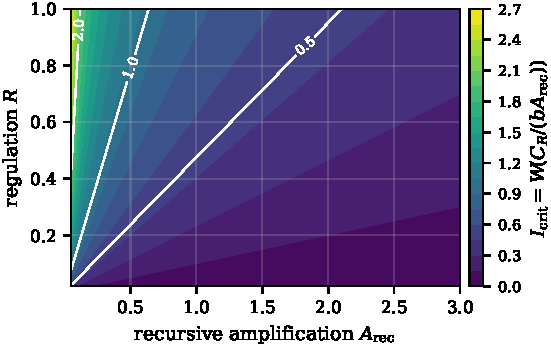
\includegraphics[width=\textwidth]{figures/fig09_lambert_boundary.pdf}
\caption{The auxiliary Lambert boundary $\Icrit$ against recursive amplification,
at five fixed values of regulatory capacity, from Eq.~\eqref{eq:Icrit}. More
regulation raises the critical capability that can be absorbed; stronger
recursive amplification lowers it, and does so steeply at small $\Arec$. This is
a diagnostic evaluated under the auxiliary balance of Eq.~\eqref{eq:CR}, not a
bifurcation set of the integrated system.}
\label{fig:lambert}
\end{figure}

\subsection{Why keep it at all}

Three reasons. It gives an analytic handle on the intuition that regulation can
only absorb so much recursive amplification. It makes the comparison between
regulatory capacity and amplification pressure explicit and plottable. And,
reported honestly, it is a worked example of the discipline the rest of the
framework demands: a candidate piece of mathematics, tested to see whether it was
really required, and found to be required only under an assumption we then have
to declare out loud.
